\documentclass{article}

\usepackage[utf8]{inputenc}
\usepackage{textcomp}
\usepackage{graphicx}
\usepackage{amssymb}
\usepackage{amsmath}
\graphicspath{ {./images/} }
\usepackage[T1]{fontenc}
\usepackage{geometry}
\usepackage{fancyhdr}
\usepackage{url}
\geometry{legalpaper, portrait, margin=0.8in}
\usepackage[font=small,labelfont=bf,tableposition=top]{caption}


\title{Computer Vision}
\author{Leonor Furtado 20190308}
\date{March 2020 - ?}

\begin{document}


\maketitle
\paragraph{Abstract}
\paragraph{}
Abstract 

\textbf{Keywords: Permafrost; Remote Sensing; Multispectral Imaging (MSI); Machine Learning; Deep Learning; Artificial Intelligence; Convolutional Neural Network (CNN); Computer Vision}

\section{Introduction}

\paragraph{}
Over the last decade, the use of Deep Learning (DL) algorithms for remote-sensing imagery has risen in popularity, mainly due to the increased availability and scale of remote sensing data.

This has been exacerbated in the last few years by open-source multi-spectral high spacial resolution data. An example of such data, which we will be using in this project, is that provided by Sentinel-2 [ref]. Sentinel-2 is a European mission from the Copernicus Programme that deployed two twin satellites in the same orbit 180 degrees apart, their optical sensors sample 13 spectral bands across an orbital swath width of 290 km (these will be described in detail in section x.x.x).

\paragraph{}
Deep Learning in remote sensing has been used in a wide range of applications many of which have been capture in a recent review study including but not limited to land use and land cover (LULC) classification, image fusion, image registration, object detection, scene classification and image segmentation.\cite{MA2019166}

The use of remote sensing imagery isn't even novel in documenting the changes in permafrost regions, where it has been widely used for decades, however the use of deep learning for this particular use case has not been widely studied. 

\paragraph{}
Permafrost is found mainly in the Arctic region, where it covers a quarter of the Northern Hemisphere's land \cite{OLTHOF2015194}. The carbon content stored in the frozen ground is thought to be double that in the atmosphere \cite{climatechange12}. As this frozen ground thaws due to global warming and other climate-change driven events, the stocks of carbon get released into the atmosphere.

\paragraph{}
The thaw of permafrost (degradation) can not only lead to damage to roads and other man-made infrastructures but also lead to the release of said trapped Green House Gases (GHGs) which consequently could contribute further to global warming and even more permafrost degradation \cite{MURTON2021857} as it warms and thaws at a faster rate, creating a vicious cycle of global warming.

This release of GHG emissions is estimated to cause extra global costs of climate-change impacts of dozens of trillions of dollars in the next two to three decades \cite{climatechange34}. 

\paragraph{}
Although little can be done to prevent permafrost degradation, the ability to identify it in a semi-automated way will go a long way in helping anticipate its impacts, taking them into account when forecasting GHG emissions and developing mitigating responses accordingly \cite{monitoringperma}.

\paragraph{}
This project aims to combine remote sensing multi spectral imagery (MSI) data with the advancements of deep learning frameworks to construct an automated way of helping to identify signs of the patterns and processes associated with permafrost degradation.


\subsection{Project Objectives and Research questions}
\paragraph{}
This project has the primary aim of using remote sensing multispectral imagery to build a deep learning neural network that allows the identification of retrogressive thaw slumps in an attempt to assess the thawing of permafrost in the Arctic.

\paragraph{}
In order to achieve this goal, this project aims to answer the following questions:

\begin{enumerate}
    \item How to deal effectively with the challenge of extracting and pre-processing multi-spectral imagery?
    \item How well can different CNN meta-architectures perform on remote sensing imagery?
    \item What is the impact of changing hyperparameters and input parameters in the different meta-architectures?
    \item Is it possible to achieve satisfactory results using only 10 meter resolution imagery, or is higher resolution needed?
\end{enumerate}

\paragraph{}

\subsection{The task of identifying retrogressive thaw slumps (RTSs) using remote sensing data}
\paragraph{}
The use of remote sensing imagery to analyse and monitor retrogressive thaw slumps (RTSs) has been widespread for many decades for many use cases in remote regions where RTSs are more commonly found. Its popularity may be due to the reduced cost and ease of data collection.
\paragraph{}
Up until the last 5 years, most techniques used to identify RTSs were traditional statistical methods or conventional machine learning techniques such as Linear Regression, Random Forest amongst others.

Nitze et al. \cite{articleing2018} take remote sensing data and apply Linear Regression and Random Forest techniques to classify RTSs and other types of Permafrost Region Disturbance (PDR).

\paragraph{}
However, since 2018, Huang et al. \cite{HUANG10122067} \cite{HUANG2020111534} \cite{HUANG2021102399} makes use of Deep Learning techniques to identify RTSs, making unprecedented contributions to the field of RTS development by using DeepLabv3+ to assign a label to each pixel in satellite images taken by the Planet CubeSat constellation.

\paragraph{}

\subsubsection{The relevance of identifying RTSs using Deep Learning and remote-sensing imagery}
\paragraph{}

Nitze et al. \cite{articleing2018} highlight the uncertainty of the scale of permafrost degradation at a rapid pace is a result of most permafrost region disturbances (PRD) not being documented due to their under-representation in the remote sensing studies. 
They also expect permafrost to degrade faster than the current projections by models that don't consider PRD-driven thaw. These models don't take into account the full extent of increased carbon emissions from permafrost thaw, which can further contribute to global warming, a.k.a. permafrost carbon feedback \cite{articlecarbonfeedback}.

In \cite{book1} the case for the need of more research targeted at identifying and monitoring PRDs for the benefit of GHG monitoring and the estimation of the consequences of it's monitoring on global warming and the future of life on earth is well argued.

\paragraph{}
Despite the extensive literature of using remote sensing imagery and Deep learning in the field of Land Cover and Land Use, it is very limited when it comes to the identification of permafrost disturbances.
A recent review study on remote sensing for permafrost related analysis \cite{rs13061217} found that only a handful amongst 325 articles in the last two decades actually used Deep Learning for permafrost-related analysis, and only one by Huang et al. \cite{HUANG2020111534} refers to RTSs in particular. 

\paragraph{}
By developing a project with researchers from both the Alfred Wegener Institute and Stockholm Environment Institute the feasibility of using DL for the identification of RTSs the relevance of this project became clear.

This project aims to make a significant contribution to this field by attempting to fill some knowledge gaps in RTS identification and provide a basis for future carbon emissions estimations.

\subsubsection{Challenges and Opportunities}
\paragraph{}
- Challenges: limited amount of labelled data, small ROI given spacial resolution 10 m per pixel

- Opportunities: Labelled data by scientists in the area availability of models trained on land use which could be used for transfer learning


\subsection{Report Structure}
\begin{itemize}
    \item Section 2 will consist of the theoretical context of this project. \item Section 3 will describe the chosen methodology, including the chosen technology and algorithms. 
    \item Section 4 will describe the chosen data and the preprocessing steps associated with it. 
    \item Section 5 will describe the experiments conducted in the optimisation of the model of choice.
    \item Section 6 will be dedicated to the final model, and it's testing evaluation.
    \item Section 7 will be composed of the final deployment and application for ease of use of citizen data scientists.
    \item Section 8 will summarise the conclusions of this project, it's limitations and suggestions for future work.

\end{itemize}

\section{Theoretical Context}
\paragraph{}
All the necessary scientific concepts and ideas will be discussed in this section to provide the reader with a theoretical context of the task at hand.

\subsection{Permafrost and its degradation}
\paragraph{}
Permafrost is characterised as frozen ground that has a temperature colder than 0 degrees C continuously for 2 or more years. Regions can be classified according to the percentage of permafrost present in the area: continuous, discontinuous, boundary. 

As the Arctic has warmed twice as fast as the globe on average, a.k.a. Arctic amplification \cite{climatechangefur} the consequences of global warming are disproportionally felt in the Arctic. 

\paragraph{}
In the Northern Hemisphere, huge amounts of soil organic carbon are trapped in permafrost soils. Any change in boundary conditions which causes the ground to warm will result in the thaw of permafrost. These abrupt thaw processes will expose previously frozen soil organic matter, causing it to undergo microbial degradation, and release GHGs as a result.Therefore, it is imperative to monitor and predict the volume of GHGs released into the atmosphere due to abrupt thaw of permafrost.

\paragraph{}
The extent of permafrost and its degradation is difficult to measure and historically requires extensive, costly investigation.A way to attempt this is to look for evidence of the formation of thermokarst landforms such as those depicted in Figure 1 which cause visible geological changes in close range of abrupt thaw locations.

\paragraph{}
Thermokarst is the  sinking of the ground's surface due to thawing of the ground (permafrost degradation). There are many examples of thermokarst landforms, amongst the most common and fast changing are lakes and ponds which amongst the fastest changing landscapes \cite{thawpic}.

In Figure 1, we can also see other examples such as active layer detachment and retrogressive thaw slump (RTS), this paper will focus on the identification of the latter in an attempt to capture some extent of permafrost degradation in the Arctic.

    \begin{figure}[hbt!]
        \centering
        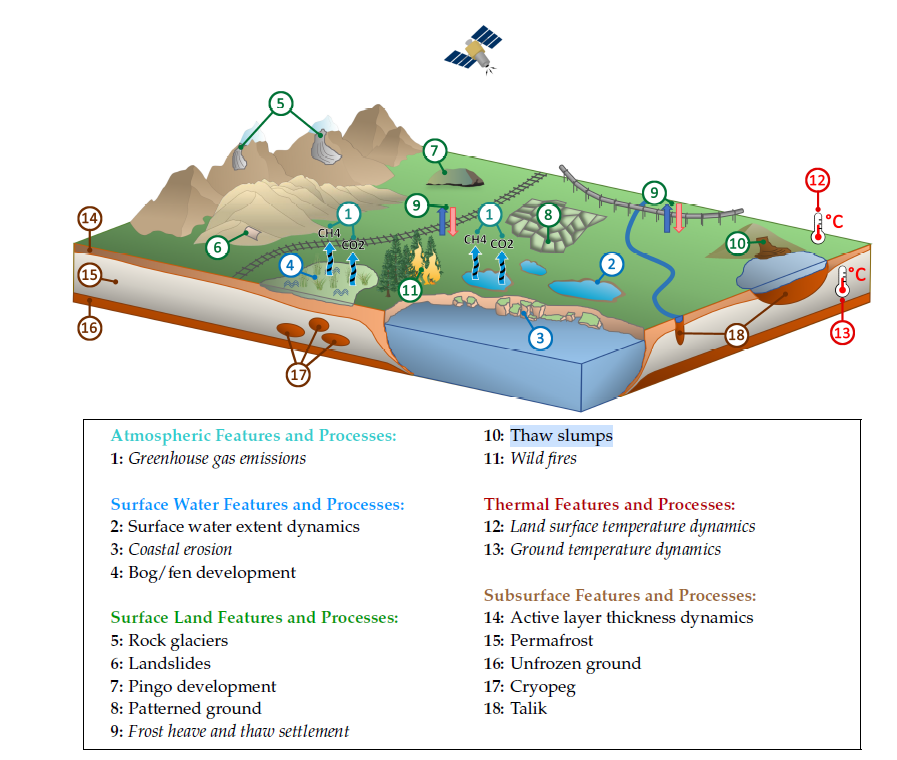
\includegraphics[width=1 \textwidth]{fig 1 thermokrast landform.png}
        \caption{Landscape features and processes info-graphic \cite{rs13061217}}
    \end{figure}

\paragraph{}
The thaw of permafrost (degradation) can not only lead to damage to roads and other man-made infrastructures but also lead to the release of said trapped Green House Gases (GHGs) which consequently could contribute further to global warming and even more permafrost degradation \cite{MURTON2021857} as it warms and thaws at a faster rate, creating a vicious cycle of global warming.

\subsubsection{Retrogressive Thaw Slump (RTS)}

\paragraph{}
RTSs can usually be described as horseshoe shaped landslides caused by the thawing of ice-rich permafrost, which causes erosion mostly at its steep head scarp. RTSs usually occur on sloped terrain so that the thawed material can flow downslope, usually into nearby water features such as lakes and rivers. \cite{articleperma}
 
 \paragraph{}
This means that RTSs have particular parts that can ease their visual identification through the mentioned head scarp, the headwall that forms after the slump, the slump floor itself \cite{LANTUIT200884} which is also described as slump scar zone. 

As some sections of the slump scar stabilise they become vegetated \cite{KOKELJ201556} and thus harder to identify using only visual Red (R), Green(G) and Blue (B) channels this is where remote sensing's other "sensor" bands can identify other features not seen with the "naked eye" \cite{HUANG2020111534}


\subsection{Artificial Intelligence Applications in Remote Sensing}
\paragraph{}
Given the lack of research found on the specific task of identifying RTSs using remote sensing imagery, a more expansive approach on looking at Deep Learning and Machine Learning (ML) techniques using RS imagery was taken.

\subsubsection{Conventional Machine Learning applications in Remote Sensing}

\paragraph{}
In a study \cite{isprs-archives-XLII-3-79-2018} on extracting built-up areas from Sentinel-2 RS imagery, Deep Learning techniques were compared against the most widely used conventional ML methods in RS classification, both Gaussian Support Vector Machines(SVM) and Back-Propagation Neural Networks(BPNN) were evaluated.

\paragraph{Support Vector Machines}
\paragraph{}
According to a 2010 review \cite{MOUNTRAKIS2011247} of over 100 studies on the use of SVM in remote sensing, this model's popularity in the field came from its ability to generalise well even when there is limited training data, which is quite common in remote sensing problems. Their major limitation comes in the form of parameter assignment issues, which affect the quality of the results.

\paragraph{Random Forests}
\paragraph{}
Random Forest (RF) has always been a popular method, as it is an ensemble classifier that makes use of multiple decision trees combined with random subsampling of the training data and variables. 
\paragraph{}
According to a review on the use of RF in remote sensing, \cite{BELGIU201624} RF became a popular classifier in RS due to the high accuracy of its classifications. It also seems to successfully handle the high dimensionality and multicollinearity of remote sensing data, as well as, being fast and not prone to overfitting. Its main limitation is its sensitivity to the sampling design.

\paragraph{Back-Propagation Neural Networks}
\paragraph{}
The traditional BPNN is a popular ML algorithm, according to a review \cite{YUAN2020111716} in environmental remote sensing it has been used extensively for research in this field. Yuan et al. reports improvement in accuracy against traditional regression methods across a number of papers by using BPNN, but highlights a couple of limitations: the slow convergence of the algorithm and how much it is affected by weight initialisation being susceptible to getting stuck in local minimums. 

\paragraph{}
This traditional Neural Network forms the back-bone of many deep learning models, so it is important to understand its inner works.

\paragraph{}

A Back-Propagation neural network consists of one or more hidden layers between an input and an output layer, each layer having many neurons/nodes that are fully connected to the next layer as it can be seen from Figure 4.  It is trained via forward and backward propagation, that is: starting with forward propagation, the input is propagated through the hidden layers in the network until it reaches the output layer where the error between the predicted and actual values is calculated. Straight after the error is calculated, it is propagated backwards to update the neuron weights of each layer with the objective of minimising the error.

    \begin{figure}[hbt!]
        \centering
        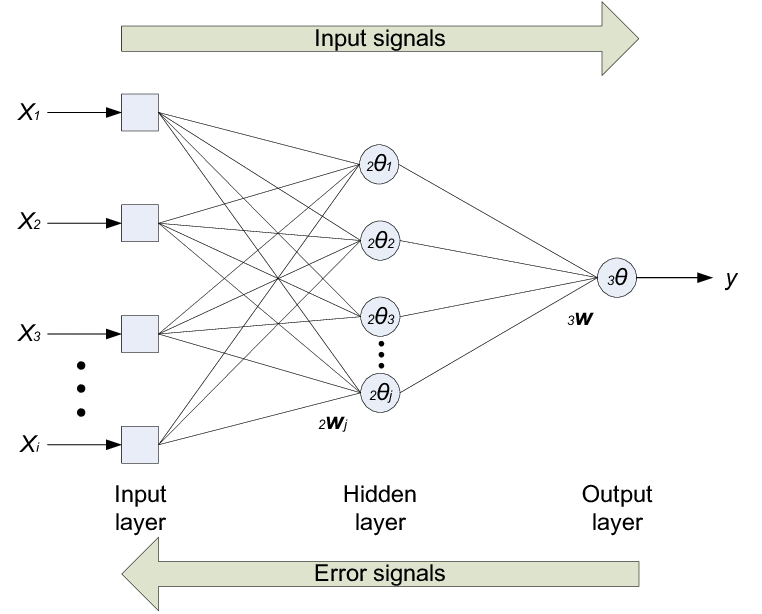
\includegraphics[width=0.5\textwidth]{Three-layer-back-propagation-neural-network.png}
        \caption{Three-layer back-propagation neural network \cite{NNpic}}
    \end{figure}

\subsubsection{Deep Learning applications in Remote Sensing Imagery}

\paragraph{}
Looking at the field of DL with RS, most studies have been focused on the field of Land Use and Land Cover (LULC) classification, as suggested by a DL in Remote sensing application review \cite{MA2019166} in Figure 2. Object detection, Scene Classification and Segmentation (a.k.a. pixel-wise classification) are also techniques to classify images or areas of these images, a detailed explanation of each of these will be given in Section 2.3.1.

    \begin{figure}[hbt!]
        \centering
        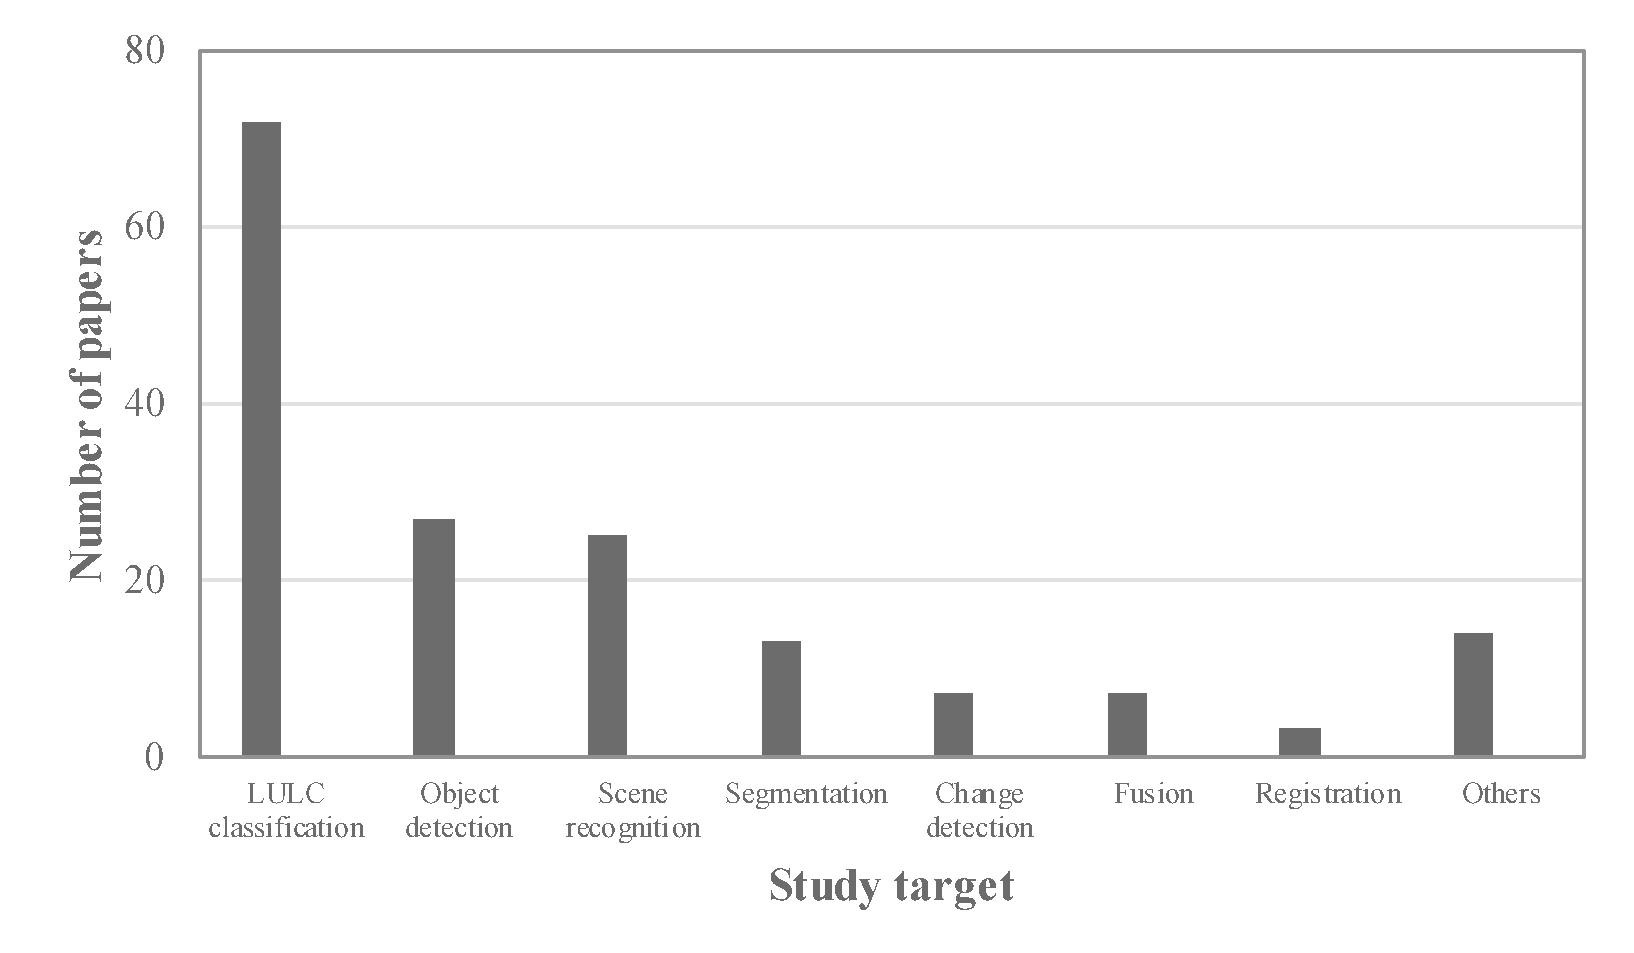
\includegraphics[width=0.75\textwidth]{study_target_ma.jpg}
        \caption{Study target of DL in Remote Sensing studies \cite{MA2019166}}
    \end{figure}

\paragraph{}
In traditional natural images, image classification the task of assigning a label to a whole input image, either by outputting a class or a probability of tasks that describe said image, however this is not the case in remote sensing, therefore there is a need to clarify the below concepts.

In remote sensing, the concept is broader, referring to either pixel-wise or "scene" classification, as shown in Figure 5.

    \begin{figure}[hbt!]
        \centering
        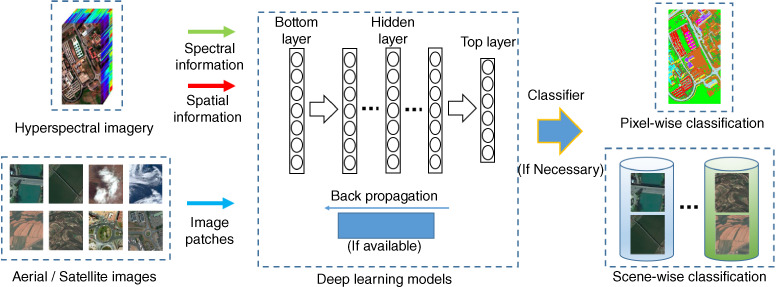
\includegraphics[width=0.75\textwidth]{widm1264-toc-0001-m.jpg}
        \caption{General Framework of Remote Sensing Image Classification Based on Deep Learning \cite{https://doi.org/10.1002/widm.1264}}
    \end{figure}


\paragraph{Pixel-wise classification} The classification of each pixel, similar to the concept of image segmentation, as it is known when performed in natural images. If we think about it conceptually, each pixel in a remote sensing image could represent, as an example, a 10 by 10 meter area, which would usually be associated with a natural image area. So by classifying each pixel in a remote sensing image, we are indeed classifying an image of 10x10 meter area. 

\paragraph{Scene classification} The automatic assignment of a semantic label to a scene. A scene being a local image patch, usually manually extracted from large-scale satellite images that contain classes (e.g. forest areas, residential area.)\cite{https://doi.org/10.1002/widm.1264}.

\paragraph{Object detection} In remote sensing images, it is used to find out if a satellite image has one or more objects belonging to a given class and find the position of each object predicted in the image.\cite{CHENG201611}

\subsubsection{Deep Learning Models in Remote Sensing}
\paragraph{}
The same review \cite{MA2019166} also suggests that the most used Deep Learning model in Remote Sensing imagery is Convolutional Neural Networks (CNN) as indicated in Figure 3.
    \begin{figure}[hbt!]
        \centering
        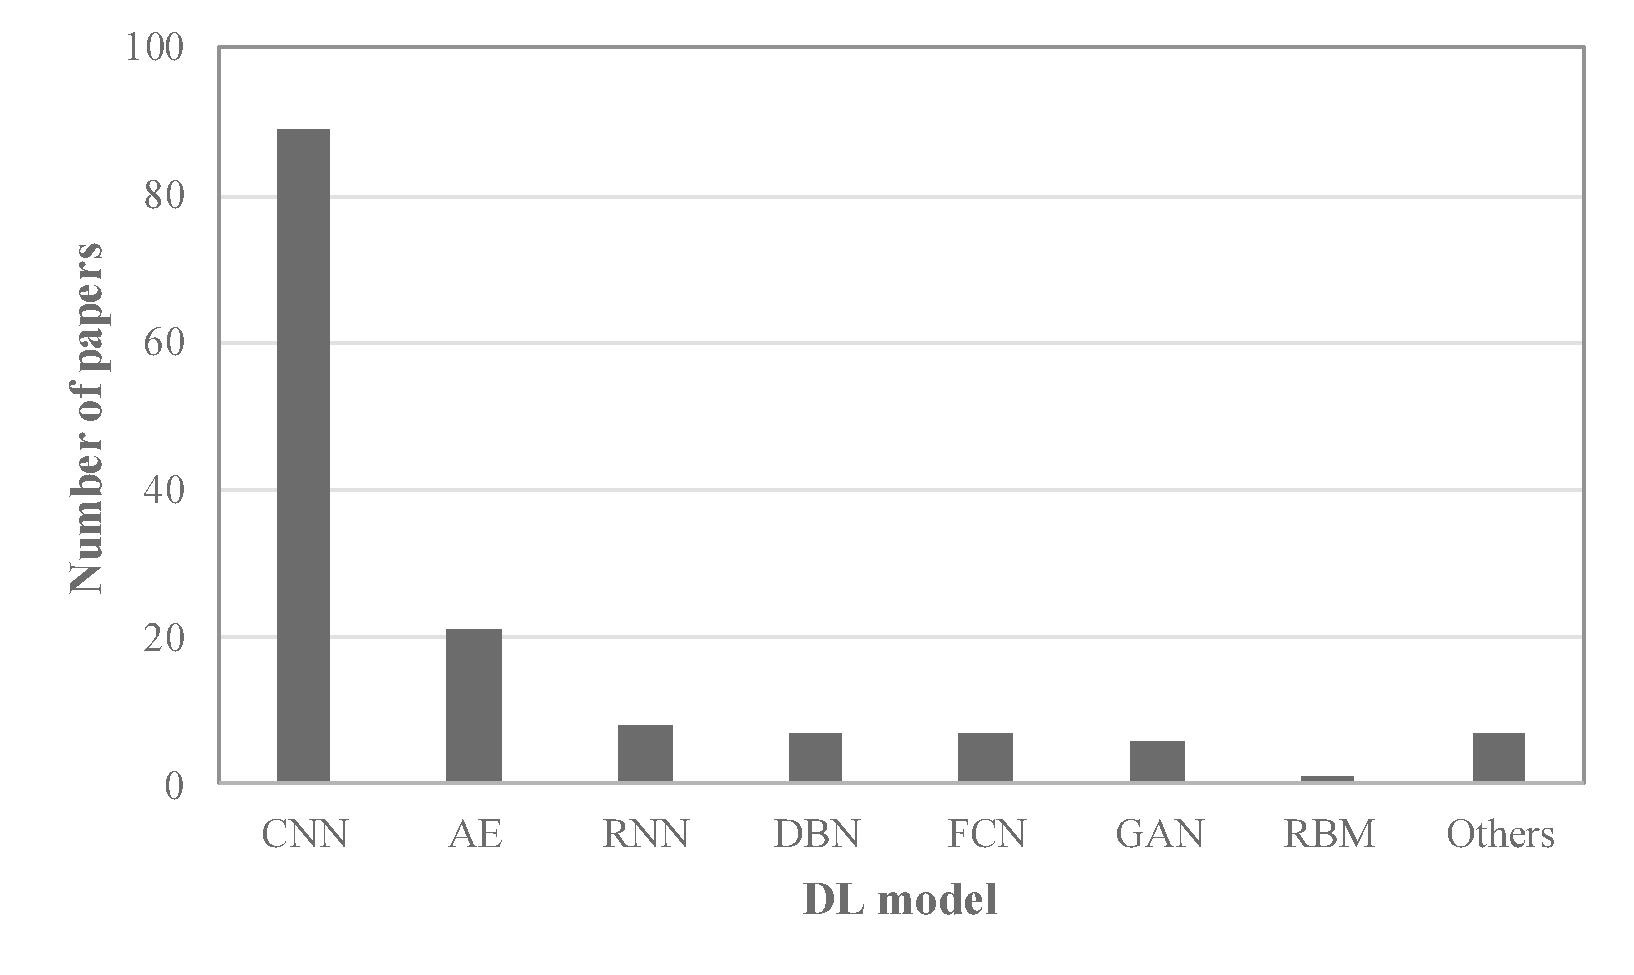
\includegraphics[width=0.75\textwidth]{DL_MA.jpg}
        \caption{DL models used in Remote Sensing studies \cite{MA2019166}}
    \end{figure}
    
\paragraph{}
CNNs, Recurrent Neural Network (RNN) and Fully Convolutional Networks (FCN) are supervised DL models, whereas Autoencoders (AE), Deep Belief Networks (DBN), Generative Adversarial Networks (GAN) models are unsupervised DL models. 
%Expand on these?     
% \paragraph{Auto Encoders}
% \paragraph{Deep Belief Networks} 
 % \paragraph{RNN}  
    
\paragraph{}
Supervised models require labelled data to learn from the ground-truth, whereas unsupervised ones don't.  As labelled data has been collected for this project, its focus will be on a supervised DL Model. CNNs have been chosen as these are the most popular supervised techniques, Section 2.4 will expand on these.

\subsection{Convolution Neural Networks (CNN)}
\paragraph{}

Convolutional Neural Networks (CNNs) are a type of Artificial Neural Networks (ANNs) that has been praised for its contribution to the field of computer vision. CNNs have been very successful  and efficient in image classification, object detection and many other applications.
\paragraph{}
In general, a CNN takes an input image, extracts low level features and hierarchically builds on this to extract more abstract features, so that it is able to extract features that are common for all outputs. This concept has its origin in the biology of the visual cortex, which has small regions of cells that "light up" to specific characteristics of the visual field until the entire visual field is processed and categorised.

\subsubsection{Main Layers of a CNN}
\paragraph{}
Like any other Neural Network, a CNN is composed of an input layer, an output layer and several hidden layers connecting them as shown in Figure 2.

The input layer usually consists of a representation of the input image to be analysed, and the output layer of the probabilities for each class.
The hidden layers usually consist of convolutional, non-linearity, pooling and fully connected layers, which are the building blocks for most CNNs and therefore will be described in detail below.

    \begin{figure}[hbt!]
        \centering
        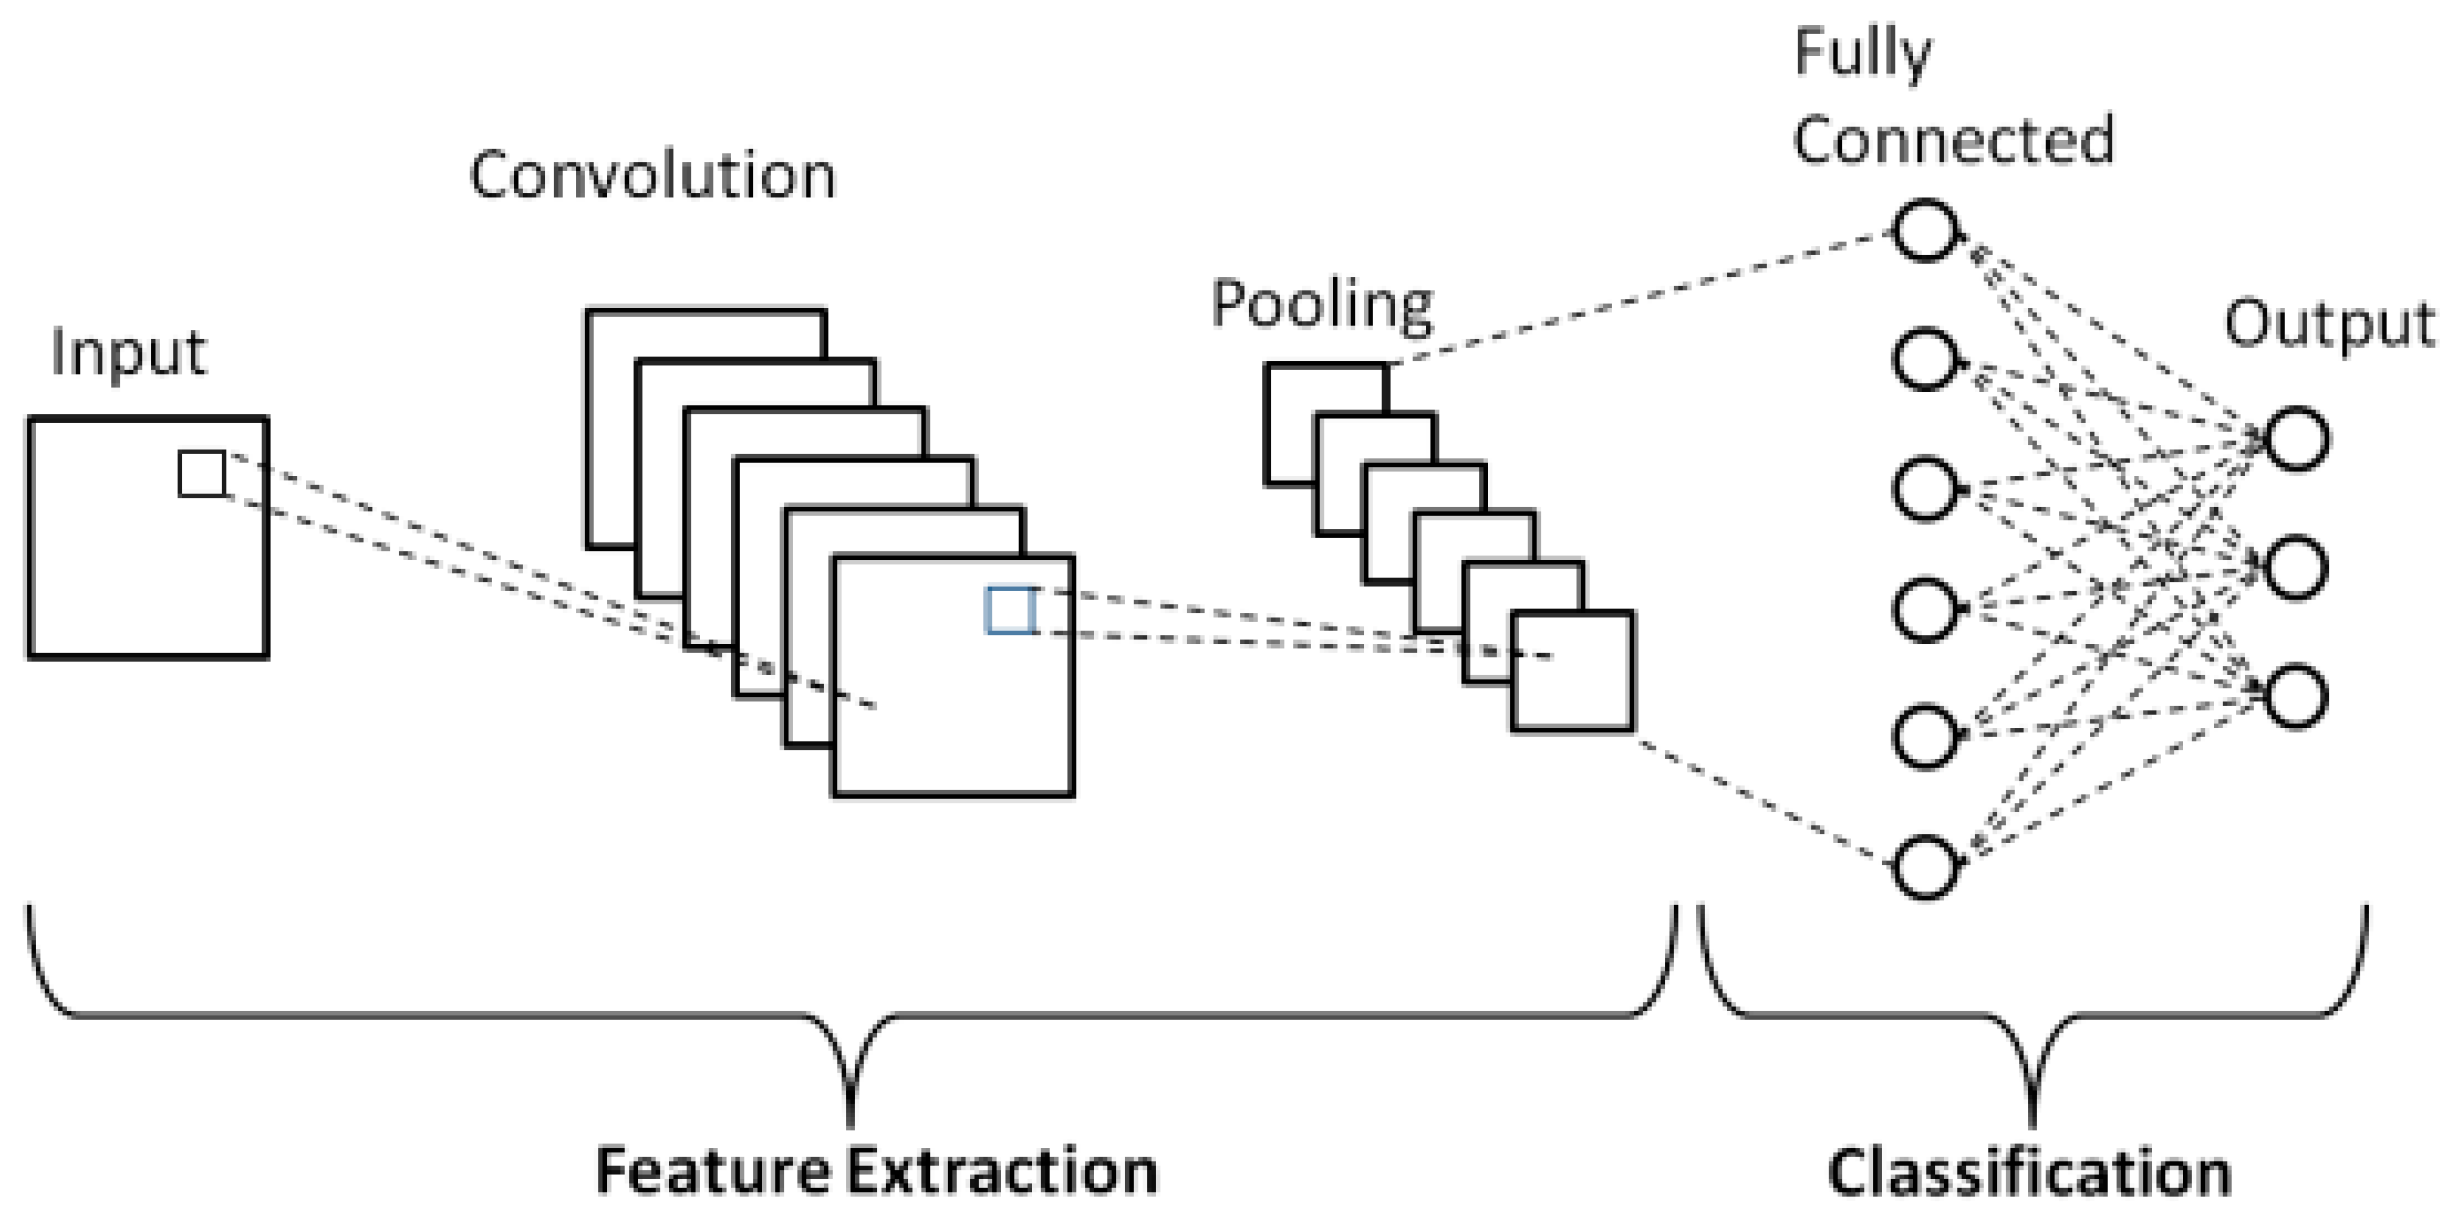
\includegraphics[width=0.75\textwidth]{cnnclassification.png}
        \caption{The main layers of a CNN \cite{10.6109/JICCE.2018.16.3.173}}
    \end{figure}

\paragraph{Input Layer}
\paragraph{}
Each image is represented as a 3D matrix with dimensions of height, width and depth. In the field of natural images the third dimension, depth, may take the value of 3 for Red, Green, Blue (RGB) channels of images, or one for grey colour images. However, in the field of remote sensing imagery this dimension can have N channels each associated with readings from a different sensor, For example Sentinel-2 images have 13 channels, this will be explored in detail in section X. 

\paragraph{Convolutional Layer}
\paragraph{}
The objective of the Convolution Operation, after which the layer has been named, is to extract features from an image. It is the key differentiator from a Dense layer, as it enables the ability to capture dependencies between pixels through the application of filters. It learns local patterns rather than global patterns.
In abstract mathematical terms, it takes the matrix of the image and the matrix of a filter/kernel and merges the information in both. By making the filter smaller than the input dimension, sparse interaction can be achieved, reducing the memory requirements and improving the model's statistically efficiency.

\paragraph{}
It also means that neurons are constrained to using the same set of weights for getting the output, a.k.a. shared parameters. This parameter sharing gives the Convolution Operator the property of translation equivariance, meaning that if we translate the input the output will also be translated, giving CNNs the ability to learn features regardless of their position.
\paragraph{}
A Convolutional layer is a layer that applies different convolution operations to the data, making it the most essential building block of a CNN, and its most computationally expensive one as well. In order to fully understand this process, it will be broken down below.

The filter/kernel, introduced above has dimensions (K) smaller than the input image for height and width but the same third dimension, the number of channels (n). The filter moves along the width and height of the input image, with a certain stride (s) value, performing matrix multiplication between the filter and the same dimensional portion of the image over which the filter is passing (depicted by the shaded area in Figure 3) until it traverses the entire image.

    \begin{figure}[hbt!]
        \centering
        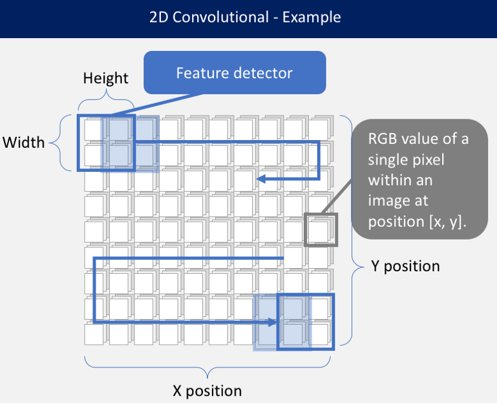
\includegraphics[width=0.5\textwidth]{2DCNN.jpg}
        \caption{The movement of the filter in a 2D CNN layer \cite{2dcnnpic}}
    \end{figure}
    
\paragraph{}   
In the case of images with n-channels the matrix multiplication is performed between the kernel and input channel stacks as depicted in Figure 4, all the results are then summed with the bias to give a one-depth channel convoluted feature map with depth equal to the number of filters (m).

    \begin{figure}[hbt!]
        \centering
        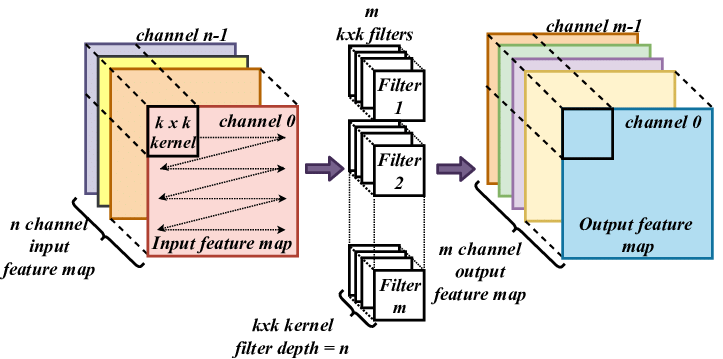
\includegraphics[width=0.75\textwidth]{Convolution-operation-in-a-CNN.png}
        \caption{The Convolution Operation in an n-channel input CNN \cite{9053228}}
    \end{figure}
    
\paragraph{}     
The size of this feature map will be affected by several parameters, some of which have been mentioned above already:

\begin{itemize}
    \item \textbf{Filter dimensions (K)} The dimensions of the filters used in the layer. For example, k x k x n in Figure 4.
    \item \textbf{Stride (s)} The number of pixels the filter shifts over the input matrix. When the stride is 1, the filters are moved 1 pixel at a time. The larger the stride, the smaller the feature map.
    \item \textbf{Number of filters (m)} The number of filters used in the convolutional layer. It is said that the higher the number of features the more image features get extracted and the better the CNN gets at recognising patterns in unseen images.
    \item \textbf{Zero Padding (p)} Sometimes the filter dimensions don't fit the image input dimensions perfectly. A strategy commonly used to maintain the input matrix dimensions and avoid the loss of information is to pad said matrix with 0s around the borders.
\end{itemize}

A CNN will usually have several convolutional layers in order to learn spatially hierarchical patterns. The first convolutional layer will learn local simple patterns such as lines and edges, then a second convolutional layer will learn features made up of the features learned in the first layer to learn more complex patterns. 

As we go deeper into the network, the filters also begin to be more responsive to a larger region of the pixel space, enabling it to learn larger patterns. The process will repeat itself for subsequent layers, the number of layers will depend on the complexity of the input image's features.

\paragraph{Non-Linearity Layer}
\paragraph{}
A non-linearity layer is nothing more than an activation function that takes the feature map generated by the convolutional layer and creates an activation map as the output. 

The different activation functions are described in section 2.3.2 in detail. Most of the recent CNN meta-architectures use Rectified Linear Units (ReLUs) (or its derivatives such as leaky RELUs) due to their efficiency and robustness to noise \cite{he2015delving}.

\paragraph{Pooling Layer}
\paragraph{}
The Pooling Layer, a.k.a. subsampling or downsampling layer, usually follows a Convolutional Layer or a Non-Linearity Layer if these are separate. Its main function is to reduce the dimensionality and subsequently the number of parameters in the network, whilst retaining the most important information of the activation map. This can reduce the training time/ computational power required and increase training efficiency through extracting the dominant translation invariant features. Just like the convolutional layer above, a window slides through each feature map applying the pooling operation, so spatial neighbourhood dimensions and stride are important parameters that need to be defined beforehand.
\paragraph{}
To achieve this there are several spacial pooling types that can be applied interchangeably, the most common ones are described below and depicted in Figure 4:
\begin{itemize}
    \item \textbf{Max Pooling} It returns the maximum value from the window of the image covered by the pooling kernel. It therefore discards noisy activations therefore performing de-noising as well as dimensionality reduction, this could help avoid overfitting. In practice, this type of pooling shows the best performance.
    \item \textbf{Average Pooling} It returns the average of all the values from the window of the image covered by the pooling kernel, only performing dimensionality reduction.
\end{itemize}

    \begin{figure}[hbt!]
        \centering
        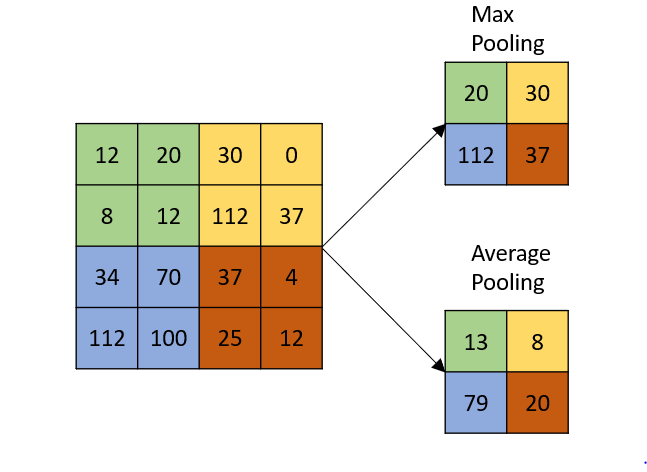
\includegraphics[width=0.5\textwidth]{pooling_diagram.png}
        \caption{The different types of Pooling}
    \end{figure}

\paragraph{Fully Connected Layer}
\paragraph{}
Finally, once the output of all the layers above successfully represent the high-level features of the input image, this output is flattened into a 1D matrix that can be fed to the Fully Connected Layers. The first few layers of this type learn non-linear combinations of these features with the objective of identifying which of these features most strongly correlate with the output classes.
\paragraph{}
To identify the most likely output class, the last of these fully connected layers usually has a softmax (multi-class problem)  or sigmoid (binary class problem) activation function to output a 1xN matrix of probabilities, with each element in this matrix corresponding to the probability of an object belonging to a specific class and all of these probabilities summing to one.


\subsubsection{Activation Functions}
\paragraph{}
There are several activation functions used for different purposes, those commonly used in hidden layers are the Tahn, Sigmoid and ReLU activation functions.
In a CNN, it is usual to have an activation function following every convolution layer to introduce non-linearity, the recommendation in modern NNs is the use of ReLU activation functions\cite{GoodBengCour16}.

We will start by introducing some activation functions commonly used in the output layer - softmax and sigmoid.

\paragraph{Softmax}
\paragraph{}
Anytime we want to represent a probability distribution over a discrete variable with K possible values we use the softmax function shown in Equation 1. It can be thought of as a generalisation of the Sigmoid function shown in Equation 2, which is used to represent it over a binary variable instead \cite{GoodBengCour16}.

\begin{equation}
    \sigma(z_i) = \frac{e^{z_{i}}}{\sum_{j=1}^K e^{z_{j}}} \ \ \ for\ i=1,2,\dots,K
\end{equation}

\paragraph{}
In Neural Networks (NN), the softmax activation function is commonly used for multi-class classification, being an output layer that predicts the multinomial probability distribution described above.

As it can be seen in Figure 6, the softmax activation will output one value for each node in the output layer, this outputted vector of probabilities that sum to 1, is interpreted as the probability of membership for each class.
\paragraph{}
\begin{figure}[hbt!]
    \centering
    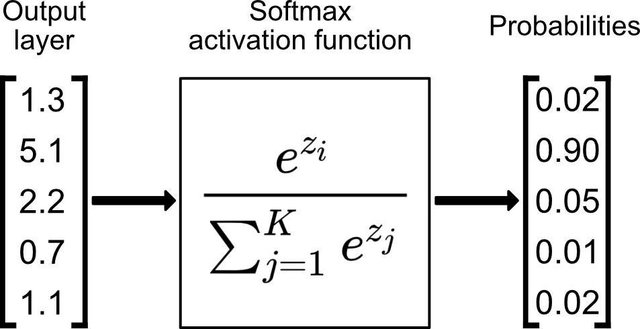
\includegraphics[width=0.4\linewidth]{softmaximg.jpg}
    \caption{Softmax activation function \cite{softmaxpic}}
\end{figure}

\paragraph{Sigmoid}
\paragraph{}
Although the Sigmoid activation function was popular in the 90s as a non-linear layer to normalise the output of each neuron in hidden layers, it lost popularity to both the activation functions that follow.

These days, since it outputs values between 0 and 1, the sigmoid activation function is usually used in the output layer for single label/ multi-label binary classification problems. 

\begin{equation}
    % sigmoid(x) = \frac{1}{1 + e^{-\alpha x}} 
    \sigma(z) = \frac{1} {1 + e^{-z}}
\end{equation}


\paragraph{Tanh}
\paragraph{}
The hyperbolic tangent activation function a.k.a. Tanh function was used as the default activation function for hidden layers in the late 90s to 2010s, after it showed signs of typically performing better than the logistic sigmoid activation function \cite{GoodBengCour16}.
Both of these activation functions are depicted in Figure 7.
\paragraph{}
As shown in Equation 3, it takes as input any real value and outputs values between -1 and 1.

\begin{equation}
    Tanh(x) = \frac{1 - e^{-\alpha x}}{1 + e^{-\alpha x}} 
\end{equation}
\paragraph{}
Despite their ability to learn complex mapping functions, both the Sigmoid and Tahn activation functions have a known limitation, they saturate for extreme values of z, only being strongly sensitive to their input when z is near 0, which can be seen from Figure 6. 

This problem is known as vanishing gradients, it makes it very difficult to know how the parameters should change to improve the cost function \cite{GoodBengCour16} and therefore for Deep Neural Networks to learn effectively.
\paragraph{}
\begin{figure}[hbt!]
    \centering
    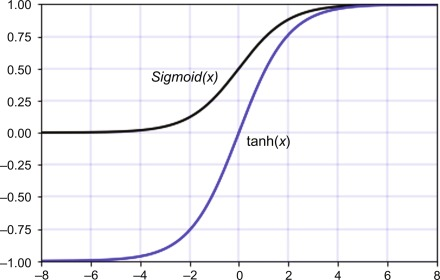
\includegraphics[width=0.5\linewidth]{tahn sigmoid funciton.jpg}
    \caption{Tahn and Sigmoid activation functions \cite{tahnfunc}}

\end{figure}

\paragraph{ReLU}
\paragraph{}
Rectified Linear Units were introduced to address this problem and quickly replaced the Sigmoid and Tahn activation functions by providing improvements in performance, Deep CNNs with ReLUs trained several times faster than the same ones with Tahn units\cite{GoodBengCour16}.

\paragraph{}
The rectified linear activation function simply returns the input value provided if this value is greater than 0, or the value 0, if the input is 0 or less.

\begin{equation}
    Relu(z) = max(0, z)
\end{equation}

\paragraph{}
In this sense, it can be said that because ReLUs are nearly linear, they preserve properties that make linear models easy to optimise and generalise well \cite{GoodBengCour16}

\paragraph{}
ReLUs don't come without limitations, large updates to the weights could mean that the input to the activation function is always negative, therefore the activation value will always be 0, this is known as the dying ReLU problem.
This means the gradient is 0, so the unit will never activate, the weights will not be adjusted, so like the vanishing gradient problem the learning will be slow with constant 0 gradients \cite{Maas13rectifiernonlinearities}.
\paragraph{}
This can be corrected by several variations of the ReLU, for example Leaky and Parametric ReLUs (PReLU) that change the slope to the left of x<0. Either by a fixed parameter in Leaky ReLU as shown in Figure 7 or by a parameter that is learned by backpropagation using weights and biases in PReLU. 

There are more complex examples like Exponential Linear Units (ELU) and Threshold ReLU functions that are known to improve accuracy compared to ReLUs.

\begin{figure}[hbt!]
        \centering
        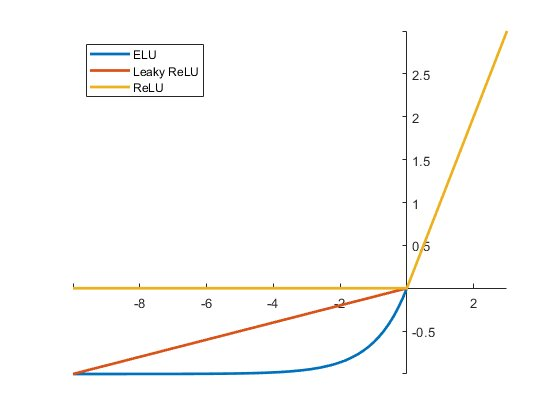
\includegraphics[width=0.65\linewidth]{RELU variations.jpg}
        \caption{Rectified Linear activation functions \cite{leakyreluimg}}
\end{figure}


\subsubsection{Classical CNN Architectures and their evolution}
\paragraph{}
In the following  subsection, the layers introduced will be arranged in the architecture first introduced by Lecun in the early 90s, followed by some other influential architectures that have built on and adapted this architecture since.
\paragraph{LeNet}
\paragraph{}
In 1989,LeCun et al. proposed the first multilayered CNN successfully trained via backpropagation. After a decade of improvement iterations, LeNet-5 \cite{726791} was the famous architecture depicted below that started the use of CNNs for Optical Character Recognition (OCR) tasks, but it didn't perform well in other computer vision problems.

    \begin{figure}[hbt!]
        \centering
        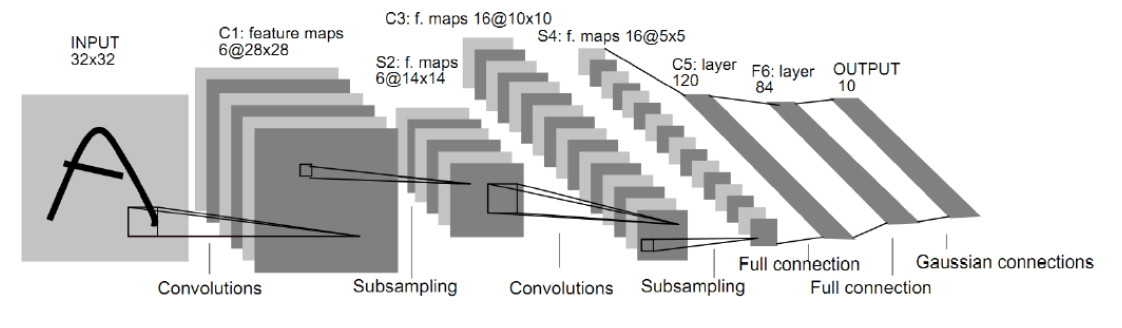
\includegraphics[width=0.75\textwidth]{lenet_arch.png}
        \caption{Architecture of LeNet-5 \cite{726791}}
    \end{figure}
    
\paragraph{AlexNet}
\paragraph{}
In 2012, Krizhevsky et al.\cite{10.5555/2999134.2999257} took LeNet's work as inspiration to create a much deeper CNN and implemented a few novel contributions which are still essential to the success of CNNs to this day:
\begin{itemize}
    \item \textbf{ReLUs} The benefits of these have been highlighted in section 2.3.2, contributing to faster training times than the Sigmoid activation function used in LeNet's implementation.
    \item \textbf{Dropout} The use of Dropout layers as a regularisation method helped avoid the problem of overfitting
    \item \textbf{Data Augmentation} Using artificial data augmentation techniques to increase the size and variety of the training dataset by translating and reflecting existing images improved the performance of the model
     \item \textbf{Training on a GPU} Using graphic processing units (GPUs) to train AlexNet allowed for faster training on great amounts of bigger images which set a milestone for the success of CNNs
\end{itemize}

    \begin{figure}[hbt!]
        \centering
        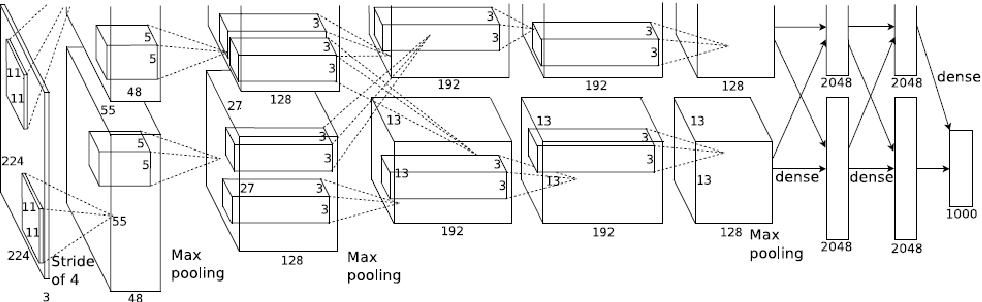
\includegraphics[width=0.75\textwidth]{alexnet_arch.png}
        \caption{Architecture of AlexNet, shows the delineation of responsibilities between 2 GPUs \cite{10.5555/2999134.2999257}}
    \end{figure}


\paragraph{VGG}
\paragraph{}
VGGNet \cite{simonyan2014deep} won the ImageNet Challenge 2014, this network built on the simple principles of the two conventional CNNs introduced above, creating a deeper network (19 weight layers) with the idea of using blocks of increasing number of filters. These repeated structures of a sequence of convolutional layers followed by a max pooling layer for downsampling, create deeper networks with more non-linearities captured. Several other factors contributed to its success:

\begin{itemize}
    \item \textbf{Filters with smaller dimensions} By using filters with a smaller receptive field of 3x3 and maintaining the number of filters in each of the convolutional layers in the same block, in a sequence of layers, more non-linearities can be captured using fewer parameters
 
    \item \textbf{Increasing number of filters} By roughly doubling the number of filters in each block, more complex features can be captured
    \item \textbf{Scale jittering} Uses scale jittering as one of the data augmentation techniques

\end{itemize}


\paragraph{Other evolutions}
\paragraph{}
Several meaningful contributions were made by other architectures, such as:

\begin{itemize}

    \item \textbf{Network in Network (NiN) \cite{lin2014network}} The main idea behind a NiN block is to apply a fully-connected layer to each pixel, they consist of a convolutional layer and multiple 1x1 convolutional layers, this design has influenced many other CNN designs
 
    \item \textbf{GoogleNet \cite{7298594}} Also working with blocks, each of its "Inception" blocks has 4 paths, extracting information in parallel through convolutional layers of different filter dimensions and max pooling layers. It also makes use of the 1x1 convolution introduced in NiN to reduce channel dimensionality per pixel. This makes it a very efficient network architecture with low computational cost.
    
    \item \textbf{Batch normalisation \cite{ioffe2015batch}} Introduced in 2015, this method makes normalisation part of the model architecture by performing it for each training mini-batch. It  not only allows the use of much higher learning rates and more relaxed initialisation, but it also acts as a regularisation technique.
    
    \item \textbf{ResNet \cite{he2015deep}} This architecture challenges the convention of optimising the original unreferenced functions by optimising the residual mappings instead. This way the authors manage to create residual networks with a depth of 152 layers, which is 8 times deeper than VGG net whilst keeping a lower complexity, making them more accurate and easier to optimise. 
    \item \textbf{DenseNet \cite{8099726}} This architecture builds on the concept of the ResNet but instead of adding inputs and outputs together in its cross-layer connections, it concatenates them instead. It also uses transition layers (1x1 convolution) to keep the dimensions under control.

\end{itemize}

% \subsection{The various CNN Architectures used in remote-sensing applications}

% \subsubsection{Fully Connected Convolutional Networks (FCCN)}
% \subsubsection{U-NET}
\paragraph{}
\paragraph{}

\paragraph{}
\paragraph{}


\bibliography{bibliography.bib}
\bibliographystyle{plain}

\end{document}